\begin{centering}

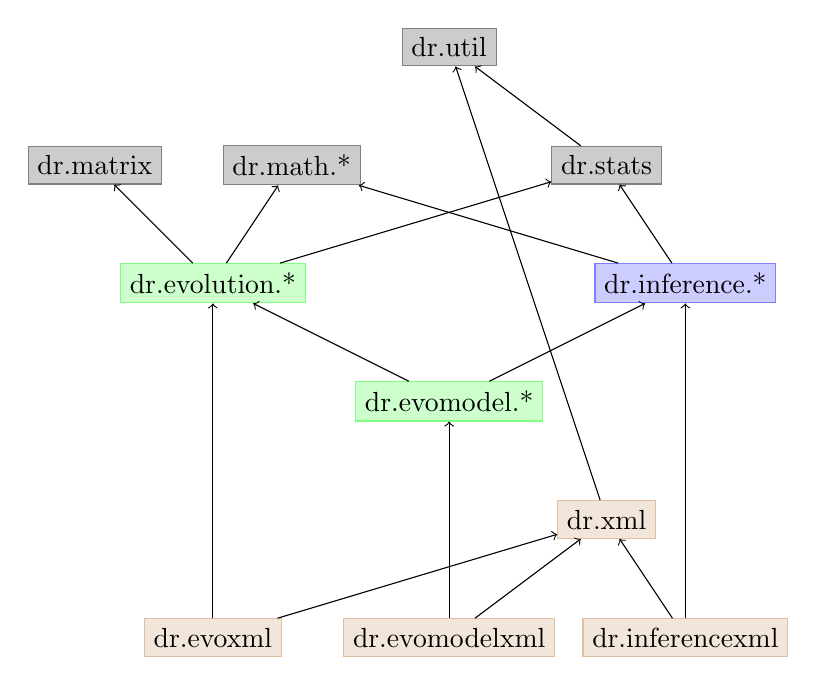
\begin{tikzpicture}[rectangle, xmlpackage/.style={draw=brown!50,fill=brown!20}, package/.style={draw=black!50,fill=black!20}, infpackage/.style={draw=blue!50,fill=blue!20}, evopackage/.style={draw=green!50,fill=green!20}]

\node[xmlpackage] (evomodelxml) at (0, -3) {dr.evomodelxml}; 
\node[xmlpackage] (evoxml) at (-3, -3) {dr.evoxml}; 
\node[evopackage] (evomodel) at (0, 0) {dr.evomodel.*}; 
\node[evopackage] (evolution) at (-3, 1.5) {dr.evolution.*}; 
\node[xmlpackage] (inferencexml) at (3, -3) {dr.inferencexml}; 
\node[infpackage] (inference) at (3, 1.5) {dr.inference.*}; 
\node[package] (stats) at (2, 3) {dr.stats}; 
\node[xmlpackage] (xml) at (2, -1.5) {dr.xml}; 
\node[package] (util) at (0, 4.5) {dr.util}; 
\node[package] (math) at (-2, 3) {dr.math.*}; 
\node[package] (matrix) at (-4.5, 3) {dr.matrix}; 

\draw [->] (inferencexml) -- (inference); 
\draw [->] (inferencexml) -- (xml); 
\draw [->] (evoxml) -- (evolution); 
\draw [->] (evoxml) -- (xml); 
\draw [->] (evomodelxml) -- (evomodel); 
\draw [->] (evomodelxml) -- (xml); 
\draw [->] (evomodel) -- (inference); 
\draw [->] (evomodel) -- (evolution); 
\draw [->] (inference) -- (math); 
\draw [->] (inference) -- (stats); 
%\draw [->] (inference) -- (xml); 
\draw [->] (evolution) -- (math); 
\draw [->] (evolution) -- (matrix); 
\draw [->] (evolution) -- (stats); 
%\draw [->] (evolution) -- (xml); 
\draw [->] (xml) -- (util); 
\draw [->] (stats) -- (util); 

\end{tikzpicture} 

\end{centering}